\documentclass[conference]{IEEEtran}
\usepackage{times}

% numbers option provides compact numerical references in the text. 
\usepackage[numbers]{natbib}
\usepackage{multicol}
\usepackage[bookmarks=true]{hyperref}
\usepackage{amsmath}
\usepackage{amssymb}
\usepackage{graphicx}
\usepackage{subfigure}
\usepackage{algorithm}

\pdfinfo{
	/Author (Homer Simpson)
	/Title  (Robots: Our new overlords)
	/CreationDate (D:20101201120000)
	/Subject (Robots)
	/Keywords (Robots;Overlords)
}

\begin{document}

% paper title
\title{Optimal Measurement Scheduling for Cooperative Localization in Resource-constrained Conditions}

% You will get a Paper-ID when submitting a pdf file to the conference system
%\author{Author Names Omitted for Anonymous Review. Paper-ID [add your ID here]}

\author{\authorblockN{Qi Yan}
\authorblockA{School of Mechanical Engineering\\
Shanghai Jiao Tong University\\
Email: qi\_yan@sjtu.edu.cn\\
Student ID:515020910184}
\and
\authorblockN{Yixing Wen}
\authorblockA{School of Mechanical Engineering\\
Shanghai Jiao Tong University\\
Email: xxx@sjtu.edu.cn\\
Student ID:5150209101xx}
}


% avoiding spaces at the end of the author lines is not a problem with
% conference papers because we don't use \thanks or \IEEEmembership


% for over three affiliations, or if they all won't fit within the width
% of the page, use this alternative format:
%
%\author{\authorblockN{Michael Shell\authorrefmark{1},
%Homer Simpson\authorrefmark{2},
%James Kirk\authorrefmark{3},
%Montgomery Scott\authorrefmark{3} and
%Eldon Tyrell\authorrefmark{4}}
%\authorblockA{\authorrefmark{1}School of Electrical and Computer Engineering\\
%Georgia Institute of Technology,
%Atlanta, Georgia 30332--0250\\ Email: mshell@ece.gatech.edu}
%\authorblockA{\authorrefmark{2}Twentieth Century Fox, Springfield, USA\\
%Email: homer@thesimpsons.com}
%\authorblockA{\authorrefmark{3}Starfleet Academy, San Francisco, California 96678-2391\\
%Telephone: (800) 555--1212, Fax: (888) 555--1212}
%\authorblockA{\authorrefmark{4}Tyrell Inc., 123 Replicant Street, Los Angeles, California 90210--4321}}


\maketitle

\begin{abstract}
Localization is essential for the application of multi-robot systems.
Due to the limitations of on-board resources, the localization algorithm must consider the trade-off between accuracy and actual costs to make the feasible implementations.
In this paper, we consider the optimal measurement scheduling with respect to dynamic topology switching for a group of robots participating in cooperative localization in resource-constrained conditions.
We formulate the novel topology switching problem for CL algorithm and moreover, does not assume full-observability condition for cost-down optimization goal, as opposed to previous work.
Next, this problem which is proven to be combinatorial and NP-hard, can be solved approximately by efficient greedy algorithm due to its super-modularity property.
Finally, the effectiveness of our proposed method is validated through simulations with real-world settings.
\end{abstract}

\IEEEpeerreviewmaketitle

\section{Introduction}
Localization plays a crucial role for successful implementation of mobile robots or mobile agents.
In recent decades, catalyzed by the work of Roumeliotis \cite{roumeliotis2002distributed}, a large number of research work focus on the localization technique for the multi-robot system (cooperative localization, CL).
Cooperative localization algorithms was intensively studied in previous work and many methods were proposed for improvement in terms of communication costs, computation costs, storage costs and localization accuracy \cite{luft2018recursive,kia2014centralizedequivalent,kia2015cooperative,vudinh2015serverclient,kia2016cooperative,chang2017multirobot,zhu2017consistent,kia2018serverassisted,razavi2018resourceaware,zhu2018loosely,chang2018optimal} but the associated costs which might be overwhelmingly high for mobile robots, were usually dismissed \cite{chang2018optimal}.
To the best knowledge, only rare papers worked on the cost-down of CL process explicitly like \cite{mourikis2006optimal,chang2018optimal}.

One way to optimize measurement scheduling for CL to lower costs without too much accuracy sacrifice is to make upper bound analysis for estimation covariance as in \cite{mourikis2006optimal,chang2018optimal}.
Riccati recursion is the key idea where the evolution of upper bound of covariance follows the Discrete-time Algebraic Riccati Equation (DARE), which could be further transformed into a continuous one, i.e. the Continuous Algebraic Riccati Equation (CARE).
The convergence of Riccati recursion, however, requires that the overall system is observable \cite{mourikis2006optimal,chang2018controltheoretical}, which means there must be at least one robot accessing absolute positioning information such as GPS or landmark  in at least an intermittent fashion \cite{mourikis2006optimal,roumeliotis2002distributed}.
Chang \cite{chang2018optimal,chang2018controltheoretical} adopted this method to lower costs of CL, such as communication and computation costs, based on their previous work on Covariance Intersection (CI) CL \cite{chang2017multirobot}.
Furthermore, in order to decouple the task of position estimation from orientation estimation, they also assumed that each robot could measure its own orientation with an a prior known variance of its measurement upper bound \cite{mourikis2006optimal,chang2018optimal}.

The full-observability assumed in \cite{mourikis2006optimal,chang2018optimal} however, is a very hard constraint for the multi-robot team and cannot be sufficed in many conditions.
This main drawback prevents the above method from actual implementation since usually the robots or agents did not receive any absolute positioning information such as in under-water situations \cite{bahr2009cooperative} and in uncharted in-door environments \cite{hausman2015cooperative,zhu2018loosely}.
Moreover, the previous work \cite{mourikis2006optimal,chang2018optimal} mainly considers the frequency of measurements or communications (if separated from relative measurements) for the CARE of corresponding Kalman filtering process, where the frequency is optimized over a continuous interval.
In actual implementation, it is usually impossible to carry out the observation process at any given frequency and it further limits the applicability of this method.

To overcome the issues of current cost-down method for CL, we propose a new algorithm from the perspective of topology switching inspired from the problem of run-time and design-time sensor selection \cite{vitus2012efficient,jawaid2015submodularity,tzoumas2016nearoptimal,tzoumas2016sensor,tzoumas2017scheduling,tzoumas2018selecting,zhang2017sensor,hausman2015cooperative}.
In \cite{hausman2015cooperative}, the authors considered the switching topology for better accuracy of	target tracking employing CL algorithm.
They mainly focused on the levels of topologies and did not quantitatively make optimization for best costs or best estimation accuracy given certain constraints.
In this paper, we consider scheduling relative measurements for a group of robots without full-observability and with process and measurement noise.
Essentially, our aim is to choose at most $k$ measurements out of all  all the possible $m$ relative measurements that could lead to the best localization accuracy, with a similar form to the sensor placement problem.
It is easily observed that the complexity of dynamic topology switching for CL is overwhelmingly high since it is a combinatorial and NP-hard problem \cite{zhang2017sensor}.
Fortunately, the logdet error corresponding to the volume of confidence ellipsoid for Kalman filtering process over a finite observation interval has the property of super-modularity \cite{tzoumas2016sensor}.
This enables us to formulate an easy greedy algorithm to give an approximate solution to the CL cost-down optimization problem. 
Moreover, a super-node server is constructed in our algorithm as in \cite{kia2018serverassisted} so as to tell each robot to take measurement from whom.
To simplify our problem at this state, some very general assumptions are made as follows: 1) the orientation measurement is accessible to each robot and only the position estimation is carried out via EKF and 2) the robot-to-server communication does not fail.

The main contributions of this paper include:
\begin{itemize}
	\item we explicitly consider dynamic topology switching method to lower the costs of CL algorithm,
	\item the full-observability condition is totally discarded as opposed to previous work in \cite{mourikis2006optimal,chang2018optimal},
	\item propose an efficient greedy approximation approach to construct the topology for best accuracy
\end{itemize}
In following sections, we would introduce the problem formulation and our proposed method.
Finally, the effectiveness of our method is validated through numerical simulations.


\section{Problem Statement}
Firstly, let us adopt the standard Extended Kalman Filter (EKF) as an benchmark to examine the \emph{Riccati recursion} based analysis.
Centralized EKF or centralized-equivalent distributed EKF \cite{roumeliotis2002distributed,kia2014centralizedequivalent,kia2016cooperative,kia2018serverassisted,luft2018recursive} would have exactly the same analysis results and for simplicity, they are all referred to \emph{CEKF-CL} in following contents.
Recall the CEKF-CL for a group of \emph{N} robots, the system model follows:
\begin{equation}
	x^i(k+1) = f^i(x^i(k),u^i_m(k))
	\label{equ::CEKF_sys}
\end{equation}
where $x^i(k) = [x_i,y_i]^T\in \mathbb{R}^{2\times1}$ is the position state vector for robot $i$, $f^i$ stands for the nonlinear system model for robot $i$, $u^i_m = u^i + \eta^i =v^i_m$ is the measured linear motion velocities with $u^i$ being the true value and $\eta^i = \eta^i_v$ the contaminating while-Gaussian noise.
The relative measurement model is written as:
\begin{equation}
	z_{ij}(k) = h_{ij}(x^i(k),x^j(k)) + \nu^i(k)
	\label{equ::CEKF_mea_rel}
\end{equation}
where $z_{i,j} \in \mathbb{R}^{2\times1}$ is the raw measurement given by sensor attached on robot $i$, $h_{ij}$ represents the measurement model and $\nu \in \mathbb{R}^{2\times1}$ is the measurement noise.
Under the assumption of system observability, the absolute positioning for is expressed as:
\begin{equation}
	z_{i}(k) = x^i(k) + \nu^i(k)
	\label{equ::CEKF_mea_abs}
\end{equation}
The system and measurement noise $\eta$ and $\nu$ respectively, are mutually independent with known variances $Q^i(k) =E(\eta^i(k)\eta^i(k)^T)$ and $R^i(k)=E(\nu^i(k)\nu^i(k)^T)$. By applying EKF over the joint system model and the measurement models, one could have \cite{kia2014centralizedequivalent,kia2018serverassisted}:
\begin{subequations}
	\begin{equation}
	\hat{x}^{i-}(k+1) = f^i(\hat{x}^{i+}(k),u^i(k))
	\label{equ::CEKF_main_xprop}
	\end{equation}
	\begin{equation}
	P^{i-}(k+1) = F^i(k)P^{i+}(k)F^i(k)^T + G^i(k)Q^i(k)G^i(k)^T
	\label{equ::CEKF_main_pprop}
	\end{equation}
	\begin{equation}
	P_{ij}^-(k+1) = F^i(k)P_{ij}^+(k)F^j(k)^T
	\label{equ::CEKF_main_corprop}
	\end{equation}
	\begin{equation}
	\hat{x}^{i+}(k+1) = \hat{x}^{i-}(k+1) + K_i(k+1)r^a(k+1)
	\label{equ::CEKF_main_xupdate}
	\end{equation}
	\begin{equation}
	P^{i+}(k+1) = P^{i-}(k+1) - K_i(k+1)S_{ab}(k+1)K_i(k+1)^T
	\label{equ::CEKF_main_pupdate}
	\end{equation}
	\begin{equation}
	P_{ij}^+(k+1) = P_{ij}^-(k+1) - K_i(k+1)S_{ab}(k+1)K_j(k+1)^T
	\label{equ::CEKF_main_corupdate}
	\end{equation}
	\begin{multline}
	K_i(k+1) = \\
	\begin{cases}
	0_{2\times2}, & \text{if no measurement} \\
	(P_{ia}^-(k+1)H_a^T + P_{ib}^-(k+1)H_b^T)S_{ab}^{-1}, &\text{if $a$ observes $b$} \\
	P_{ia}^-(k+1)H_{aa}^T S_{aa}^{-1}, &\text{if $a$ observes itself}
	\end{cases}
	\label{equ::CEKF_main_gain}
	\end{multline}
	\label{equ::CEKF_main}
\end{subequations}
where $F^i = \partial f^i (x^i,u_m^i)/\partial x^i \in\mathbb{R}^{2\times2}$ and $G^i = \partial f^i (x^i,u_m^i)/\partial \eta^i\in\mathbb{R}^{2\times1}$.
The other terms related to relative measurements $r^a,S_{ab},H_a,H_b,H_{aa}$ are further formulated as:
\begin{subequations}
	\begin{equation}
	r^a(k+1) = z_{ab}(k+1) - h_{ab}(\hat{x}^{a-}(k+1),\hat{x}^{b-}(k+1))
	\label{equ::CEKF_mea_inno}
	\end{equation}
	\begin{equation}
	\begin{split}
	S_{ab} = R^a(k+1) &+ H_a(k+1)P^{a-}(k+1)H_a(k+1)^T
	\\ &+ H_a(k+1)P_{ab}^{-}(k+1)H_b(k+1)^T
	\\ &+ H_b(k+1)P^{b-}(k+1)H_b(k+1)^T
	\\ &+ H_b(k+1)P_{ba}^{-}(k+1)H_a(k+1)^T
	\end{split}
	\end{equation}
\end{subequations}
where (assume that $a<b$)
\begin{subequations}
	\begin{equation}
	H_l(k) = \partial h_{ij}(\hat{x}^{i-}(k),\hat{x}^{j-}(k)/\partial\hat{x}^{l-}(k), l\in\{a,b\}
	\end{equation}
	\begin{equation}
	H_{aa}(k) = I_{2}
	\end{equation}
\end{subequations}
$r^a\in \mathbb{R}^{2\times1}$ and $S_{ab}\in \mathbb{R}^{2\times2}$ stand for the mean and covariance of innovation respectively. $H_a$ and $H_b$ are Jacobian matrices of relative measurement model and $H_{aa}$ stands for that of absolute measurement model.

\section{Upper Bound Derivation based on Riccati recursion}
By closely examining the propagation and update process at Eq. \eqref{equ::CEKF_main}, one could derive the upper bound $\Pi^i(k)$ of covariance evolution.
The first step is to make the upper bound of covariance $P^i$ independent of states such that its coefficients are constant as in \cite{mourikis2006performance,chang2018optimal}.
In Eq. \eqref{equ::CEKF_main}, we have:
\begin{equation*}
	P^{i-}(k+1) = F^i(k)P^{i+}(k)F^i(k)^T + G^i(k)Q^i(k)G^i(k)^T
\end{equation*}
where
\begin{equation*}
\begin{split}
F^i(k) &= \partial f^i (x^{i+}(k),u_m^i(k))/\partial x^{i+}(k)
\\ & = I_{2}
\\G^i(k) &= \partial f^i (x^i,u_m^i)/\partial \eta^i \\ &=
\begin{bmatrix}
T_p cos(\phi_i) \\
T_p sin(\phi_i)
\end{bmatrix}
\end{split}
\end{equation*}
To eliminate the state-dependent terms and obtain an upper bound, by treating $G^i(k)Q^i(k)G^i(k)^T$ altogether, we have:
\begin{equation}
\begin{split}
G^i(k)Q^i(k)G^i(k)^T
&=T_p^2\begin{bmatrix} cos(\phi_i) \\ sin(\phi_i) \end{bmatrix} {\eta_v^{i}}^2
\begin{bmatrix} cos(\phi_i) & sin(\phi_i) \end{bmatrix}
\\&\leq T_p^2 \check{Q}^i
\end{split}
\end{equation}
with $\check{Q}^i = {\eta_v^{i}}^2 I_{2}$.
So for the propagation stage, we could construct such an upper bound:
\begin{equation}
\begin{split}
	P^{i-}(k+1) \leq P^{i+}(k) + T_p^2\check{Q}^i
\end{split}
\end{equation}
It is more convenient to consider the upper bound of the aggregated covariances $P(k)\in\mathbb{R}^{2N\times2N}$, whose diagonal blocks are covariances for each agent and off-diagonal ones are correlations between agents.
First we have:
\begin{equation}
P^{-}(k+1) \leq P^{+}(k) + T_p^2 \check{Q}
\end{equation}
where $\check{Q} = \text{Diag}(\check{Q}^1,\check{Q}^2,...,\check{Q}^N)$.
Assume that $P^{+}(k)\leq\Pi^{+}(k)$, we have:
\begin{equation}
\Pi^-(k+1) = \Pi ^+(k) + T_p^2 \check{Q}
\end{equation}
such that $P^{-}(k+1) \leq \Pi^-(k+1)$.
If there is a relative measurement from robot $a$ with respect to robot $b$, we have (assume $a<b$):
\begin{equation*}
\begin{split}
z_{ab} (k) &= h_{ab}(x^a(k),x^b(k)) + \nu^a(k)
\\&= C^T(\phi_a) \left(\begin{bmatrix}
x_b - x_a \\ y_b - y_a
\end{bmatrix}\right)
+ \nu^a(k)
\end{split}
\end{equation*}
in which $C(\phi_a)$ is the rotational matrix:
\begin{equation*}
C(\phi_a) = \begin{bmatrix}
cos(\phi_a) & -sin(\phi_a) \\
sin(\phi_a) & cos(\phi_a)
\end{bmatrix}
\end{equation*}
Here under our assumption, $\phi_a$ is measured by sensors on each agent and its covariance has an a prior known upper bound.
By linearizing the previous equation, the measurement error follows:
\begin{equation}
	\tilde{z}_{ab}(k) = \tilde{H}_{ab}(k)X(k) + \nu^a(k)
\end{equation}
where
\begin{equation*}
\begin{split}
	\tilde{H}_{ab} &= \begin{bmatrix}
0_{2\times2} &... &{H}_a &0_{2\times2}&...&H_b & 0_{2\times2} & ...&0_{2\times2}
\end{bmatrix}
\\
H_a &= -C^T(\phi_a),H_b = C^T(\phi_a)
\\
X(k) &= [x^1(k)^T,x^2(k)^T,...,x^N(k)^T]^T
\end{split}
\end{equation*}
By extracting the rotational matrix, one could have:
\begin{equation}
\begin{split}
	\tilde{H}_{ab} = C^T(\phi_a)\check{H}_{ab}
\end{split}
\end{equation}
where $\check{H}_{ab} = \begin{bmatrix}
0_{2\times2} &... &\overbrace{-I_2}^a &0_{2\times2}&...&\overbrace{I_2}^b & 0_{2\times2} & ...
\end{bmatrix}$
Also, $S_{ab}$ could be rewritten as:
\begin{equation}
S_{ab}(k+1) = R^a(k+1) + \tilde{H}_{ab}(k+1)P^-(k+1)\tilde{H}^T_{ab}(k+1)
\end{equation}
Covariance update could be rewritten as:
\begin{equation}
	P^+(k+1) = P^-(k+1) - K(k+1)S_{ab}(k+1)K^T(k+1)
\end{equation}
where
\begin{equation*}
K(k+1) = [K_1^T,K_2^T,\dots,K_N^T]^T = P^-(k+1)\tilde{H}^T_{ab}S_{ab}(k+1)^{-1}
\end{equation*}
It could be turned into information filter form:
\begin{equation*}
\begin{split}
&P^+(k+1)^{-1} = \tilde{H}^T_{ab}(k+1)R^a(k+1)^{-1}\tilde{H}_{ab}(k+1) \\&+ P^-(k+1)^{-1}
\\&=\check{H}^T_{ab}(k+1)C(\phi_a)R^a(k+1)^{-1}C^T(\phi_a)\check{H}_{ab}(k+1) \\&+ P^-(k+1)^{-1}
\\& \geq\check{H}^T_{ab}(k+1)\check{R}^a(k+1)^{-1}\check{H}_{ab}(k+1) + P^-(k+1)^{-1}
\end{split}
\end{equation*}
Following the measurement covariance expression in \cite{chang2018optimal,mourikis2004analysisa,mourikis2006performance}, the above inequality holds:
\begin{equation*}
\check{H}^T_{ab}C(\phi_a){R^a}(k+1)^{-1}C^T(\phi_a)\check{H}_{ab} \geq \check{H}^T_{ab}\check{R}^a(k+1)^{-1}\check{H}_{ab}
\end{equation*}
$\check{R}^a(k+1)$ is the upper bound of measurement residual covariance at time step of $k+1$.
This type of covariance upper bound whose could be easily built as in \cite{chang2018optimal,mourikis2006performance}:
\begin{subequations}
	\begin{equation}
	R^i \leq \check{R}^i = \text{max}(\sigma_{di}^2,d_{max}^2\sigma_{\phi_i}^2) I_2
	\end{equation}
	\begin{equation}
	\text{Diag}(R^1,R^2,...,R^N)\leq \check{R} = \text{Diag}(\check{R}^1,\check{R}^2,...,\check{R}^N)
	\end{equation}
\end{subequations}
where the $\check{R}^i$ is time-invariant.
Now the upper bound of the updated covariance at time step of $k+1$ could be obtained:
\begin{equation}
\Pi ^{+}(k+1)^{-1} = \check{H}^T_{ab}\check{R}^{a}(k+1)^{-1}\check{H}_{ab} + \Pi ^{-}(k+1)^{-1}
\end{equation}
where $\check{H}_{ab}(k+1)$ is susceptible to measurement topologies and $\check{R}^a$ is a \emph{constant} matrix.
As in \cite{mourikis2006performance,chang2018optimal,chang2018controltheoretical} if there are more than one measurement at any time instance, one need to augment the rows of matrix $\check{H}_{ab}$ to $\check{H}$ so as to incorporate this measurement information.

To sum up, the upper bound evolution now follows:
\begin{subequations}
	\begin{equation}
	\Pi^{-}(k+1) =\Pi^{+}(k) + T_p^2\check{Q}
	\end{equation}
	\begin{equation}
	\Pi ^{+}(k+1)^{-1} = \Pi ^{-}(k+1)^{-1} + \check{H}^T(k+1)\check{R}(k+1)^{-1}\check{H}(k+1)
	\end{equation}
	\label{equ::UB_CEKF}
\end{subequations}
Eq. \eqref{equ::UB_CEKF} is a \emph{Riccati recursion} apparently, with similar form as in \cite{mourikis2006performance,chang2018optimal,chang2018controltheoretical}.
The last equation is equivalent to
\begin{equation}
\begin{split}	
	\Pi ^{+}(k+1) &= \Pi ^{-}(k+1) + T_p^2\check{Q} - \Pi ^{-}(k+1) \check{H}^T \\
	&\times (\check{H} \Pi ^{-}(k+1)\check{H}^T +  \check{R}(k+1))^{-1} \check{H} \Pi ^{-}(k+1)
\end{split}
%\begin{split}
%\bar{\Pi} &^{+}(k+1) = \bar{\Pi} ^{-}(k+1) + \bar{\Pi} ^{-}(k+1) \check{H}^T \\
%&\times (\check{H} \bar{\Pi} ^{-}(k+1)\check{H}^T +  \check{R}(k+1) + Z^{-1})^{-1} \check{H} \bar{\Pi} ^{-}(k+1)
%\end{split}
\end{equation}

\section{Scheduled Measurements with Update Threshold}
As proposed in \cite{you2012kalman,you2013kalman,wang2013sequential,wu2013eventbased,han2015stochastic}, an event-triggering update policy could be adopted for EKF estimator to reduce the communication rate with acceptably small accuracy loss.
For simplicity, this type of algorithm is referred to as \emph{TEKF-CL} (threshold EKF) hereafter.
The main idea is to determine whether the distributed sensor (here as robot agent) should send its measurements to fusion-center (FC) (or an equivalent server) or not based on some \emph{thresholds} related to measurement innovation.
Adopting the stochastic method in \cite{han2013stochastic,han2015stochastic} , one could build a similar rule for Eq. \eqref{equ::CEKF_mea_inno}. Let the scheduling variable $\gamma_k$ be
\begin{equation}
	\gamma_k = \begin{cases}
	0 &, \text{if }\zeta_k \leq \psi(z_k) \\
	1 &, \text{otherwise}
	\end{cases}
	\label{equ::TEKF_gamma_k}
\end{equation}
where $\zeta_k$ is an independent and identically distributed variable, uniformly distributed over [0,1].
$\psi(z_k)$ represents the threshold function dependent on the measurement innovation $z_k$ at time step of $k$.
\begin{equation}
	\psi(z) \triangleq \text{exp}(-\frac{1}{2}z^T Z z)
\end{equation}
with $Z$ being a positive definite matrix.
The master agent in the measurements would send its innovation to the FC if $\gamma_k =1$ and the rest procedures follow \eqref{equ::CEKF_main_xupdate},\eqref{equ::CEKF_main_pupdate},\eqref{equ::CEKF_main_corupdate},\eqref{equ::CEKF_main_gain}. Otherwise if $\gamma_k=0$, state updates would not proceed while the covariance matrices (including the correlations) still receive updates.
The general update method is described as follows:
\begin{subequations}
\begin{equation}
P^{i+}(k+1) = P^{i-}(k+1) - \gamma_k K_iS_{ab}(k+1)K_i^T
\end{equation}
\begin{equation}
P_{ij}^+(k+1) = P_{ij}^-(k+1) - K_iS_{ab}(k+1)K_j^T
\end{equation}
\label{equ::TEKF_update}
\end{subequations}
where
\begin{equation}
S_{ab} = R^a + \tilde{H}_{ab}P^-(k+1)\tilde{H}^T_{ab} + (1-\gamma_k)Z^{-1}
\end{equation}
In this stochastic event-triggering measurement scheduling, there would always be covariance updates if a measurement happens, while the state update might be omitted.
Following the analysis in \cite{han2015stochastic}, we now derive the relationship between communication rate $\gamma$ and the steady-state collective covariance upper bound $\Pi$.

Firstly, since the system is observable, the covariance upper bound in Eq. \eqref{equ::UB_CEKF} is convergent as proven in \cite{mourikis2006performance,chang2018optimal}.
For clarity, we define the following discrete-time Riccati equation:
\begin{equation}
g_W (X) \triangleq X + T_p^2 \check{Q} - X\check{H}^T( \check{H} X \check{H}^T + W)^{-1}\check{H}X
\end{equation}
If $W = \check{R}$, the above equation turns into Eq. \eqref{equ::UB_CEKF} clearly.
The convergent solution to this equation is by setting $X = g_W(X)$.
Therefore, we define the following covariance bounds.
$\bar{\Pi}$ is the unique solution to
\begin{equation}
	\bar{\Pi} = g_{\check{R}+Z^{-1}} (\bar{\Pi})
\end{equation}
$\underline{\Pi}$ is the unique solution to
\begin{equation}
\underline{\Pi} = g_{\check{R}} (\underline{\Pi})
\end{equation}
$\bar{\Pi}$ is the worse-case performance with every measurement omitted and $\underline{\Pi}$ is the best-case performance with every measurement transmitted.
Clearly $\bar{\Pi} \geq \underline{\Pi}$ holds.
Moreover, the empirically expected covariance $\Pi^*$ as defined in \cite{han2015stochastic} is adopted.
$\Pi^*$ is the unique solution to
\begin{equation}
	\Pi^* = g_{R^*}(\Pi^*)
\end{equation}
with
\begin{equation}
	R^* = (\gamma \check{R}^{-1} + (1-\gamma) (\check{R} + Z^{-1})^{-1} ) ^{-1}
\end{equation}

Second, as proven in \cite{han2013stochastic,han2015stochastic}, the communication rate is upper bounded by:
\begin{equation}
	\gamma = 1 - \frac{1}{\sqrt{\text{det}(I + (\check{H}\bar{\Pi}\check{H}^T + \check{R} )Z )}}
\end{equation}
It is observed that the rate $\gamma$ is increasing with respect to matrix $Z$ and $\bar{\Pi}$.
And $\bar{\Pi}$ is also increasing regarding $Z$.
So the only tuning parameter here is the positive definite matrix $Z$.

This technique could be further incorporated with the \emph{SA-split-EKF CL} as proposed in \cite{kia2018serverassisted,kia2016cooperative}. Let $\phi^i(0) = I_2$ and $\Pi_{ij}(0) = 0_{2\time2}$, $j\ne i$.
Assume robot $a$ takes measurement with respect to $b$.
Now for each agent $i$, let
\begin{subequations}
	\begin{equation}
	\phi^i(k+1) = F^i(k)\phi^i(k)
	\label{equ::TEKF_phiprop}
	\end{equation}
	\begin{equation}
	\Pi_{ij}(k+1) = \Pi_{ij}(k) - \Gamma_i(k+1)\Gamma_j(k+1)^T
	\label{equ::TEKF_piprop}
	\end{equation}
\end{subequations}
where
\begin{subequations}
	\begin{equation}
	\Gamma_i(k+1) = 0, \text{if there is no measurement at }k+1
	\end{equation}
	\begin{equation}
	\begin{split}
	&\Gamma_a(k+1) = (\Pi_{ab}(k)\phi^b(k+1)^TH_b^T +\\ &\phi^a(k+1)^{-1}\check{P}^{a-}(k+1)H_a^T)S_{ab}^{-1/2},\text{   if } a\overset{k+1}{\longrightarrow} b
	\end{split}
	\end{equation}
	\begin{equation}
	\begin{split}
	&\Gamma_b(k+1) = (\phi^b(k+1)^{-1}\check{P}^{b-}(k+1)H_b^T
	 +\\&\Pi_{ba}(k)\phi^a(k+1)^TH_a^T )S_{ab}^{-1/2}, \text{   if } a\overset{k+1}{\longrightarrow} b
	\end{split}
	\end{equation}
	\begin{equation}
	\begin{split}
	&\Gamma_l(k+1) = (\Pi_{la}(k)\phi^a(k+1)^TH_a^T
	+\\&\Pi_{lb}(k)\phi^b(k+1)^TH_b^T )S_{ab}^{-1/2}, l\notin\{a,b\} \text{,   if } a\overset{k+1}{\longrightarrow} b
	\end{split}
	\end{equation}
	\label{equ::TEKF_Gamma}
\end{subequations}
with $\check{P}^{l-}(k+1)$ being the modified robot-wise covariance at the server.
It is designed to cope with its update when at some previous time step $l$, $\gamma_{l} = 0$ and there is no transmitted measurement from $l+1$ to $k$.
\begin{subequations}
\begin{equation}
	\gamma_{p}(k+1) = \begin{cases}
	0, & \text{if last measurement was not transmitted} \\
	1, & \text{otherwise}
	\end{cases}
\end{equation}
\begin{equation}
\begin{split}
&\check{P}^{j-}(k+1) =
\\&\begin{cases}
	P^{j-}(k+1) - &\phi_j(k+1)\Pi_j^*\phi_j(k+1)^T ,j\in\{a,b\},
 \\& \text{if } \gamma_{p} = 0 \\
 P^{j-}(k+1), & \text{otherwise}
\end{cases}
\\&= P^{j-}(k+1) - (1-\gamma_{p})\phi_j(k+1)\Pi_j^*\phi_j(k+1)^T
\end{split}
\label{equ::TEKF_P_rec}
\end{equation}
\end{subequations}
The variable $\gamma_p$ is stored on the server to tell whether the last measurement is under threshold or not: if it is, then modify the $P^{j-}$ before using it.
It is worth noting that $\gamma_{p}$ is updated at the end of update process.
Unlike \cite{kia2018serverassisted}, now the server also needs to store $\Pi_i^*$ with space complexity of $O(N)$ to recover the under threshold update on local covariance matrices.
Similarly, we also have:
\begin{equation}
	\begin{split}
	&S_{ab} = R^a(k+1) \\&+ H_a\check{P}^{a-}(k+1)H_a^T + H_a\phi^a(k+1)\Pi_{ab}(k)\phi^b(k+1)^TH_b^T
	\\ &+ H_b\check{P}^{b-}(k+1)H_b^T + H_b\phi^b(k+1)\Pi_{ba}(k)\phi^a(k+1)^TH_a^T
	\end{split}
	\label{equ::TEKF_sab}
\end{equation}
\begin{algorithm}
	\textbf{Initialization} (k=0):\\
	Robot: $\hat{x}^{i+}(0)\in\mathbb{R}^{2\times1}, P^{i+}(0)\in\mathbb{S}^{2\times2}_{>0},\phi_i(0) = I_2$\\
	Server: $\Pi_{ij}(0) = 0_{2\times2},j\in\{i+1,...,N\}, \Pi_i^* = 0_{2\times2}$\\
	\textbf{Iteration} k\\
	1: \textbf{Propagation}: \\each robot $i$ calculates $(x^{i-}(k+1),P^{i-}(k+1),\phi^i(k+1)$ \\$\longleftarrow (x^{i+}(k),P^{i+}(k),\phi^i(k))$ using Eq. \eqref{equ::CEKF_main_xprop}, \eqref{equ::CEKF_main_pprop}, \eqref{equ::TEKF_phiprop} \vspace{1ex}\\
	2: \textbf{Update}:\\
	If there is no measurement,\\
	Robot: $\hat{x}^{i+}(k+1)=\hat{x}^{i-}(k+1), P^{i+}(k+1)=P^{i-}(k+1)$\\
	Server: $\Pi_{ij}(k+1) = \Pi_{ij}(k),j\in\{i+1,...,N\}$ \vspace{1ex}\\
	If $a\overset{k+1}{\longrightarrow}b$, robot $a$ informs the server and the server takes messages from $a$ and $b$:\\
	Msg$_a$ = $(z,\hat{x}^{a-}(k+1),P^{a-}(k+1),\phi^a(k+1))$ \\
	Msg$_b$ = $(\hat{x}^{b-}(k+1),P^{b-}(k+1),\phi^b(k+1))$ \vspace{0.5ex}\\
	Then the server computes $(\check{P}_j(k+1),S_{ab}(k+1),\Gamma_i(k+1))$ $\longleftarrow (\text{Msg}_a,\text{Msg}_b)$ using Eq. \eqref{equ::TEKF_P_rec}, \eqref{equ::TEKF_sab}, \eqref{equ::TEKF_Gamma} \vspace{0.5ex} \\
	If $\gamma_{k+1} = 1$, the server computes $\bar{r}^a = S_{ab}^{-1/2}r^a$ and sends $\text{Msg}_\text{u}^i = (\bar{r}^i,\Gamma_i,(1-\gamma_{p})\Pi_i^*)$ to robot $i$.\\
	Robot $i$ then update its state and covariance estimations:
	\begin{subequations}
		\begin{equation}
		\hat{x}^{i+}(k+1) = \hat{x}^{i-}(k+1) + \phi^i(k+1)\Gamma_i\bar{r}^a
		\end{equation}
		\begin{equation}
		\hat{P}^{i+}(k+1) = \hat{P}^{i-} - \phi^i(k+1)(\Gamma_i\Gamma_i^T+(1-\gamma_{p})\Pi_i^*)\phi^i(k+1)^T
		\end{equation}
	\end{subequations}
	Otherwise if $\gamma_{k+1} = 0$, the server does not send information to any robot but implicitly keep the updated robot-wise covariance for next update to use.
	\begin{subequations}
		\begin{equation}
		\Pi_i^* = \Gamma_i(k+1)\Gamma_i(k+1)^T
		\end{equation}
		\begin{equation}
		\gamma_{p}(k+2) = \begin{cases}
		0, & \text{if } \gamma_{k+1} = 0 \\
		1, & \text{otherwise}
		\end{cases}
		\end{equation}
	\end{subequations}
	At last, the server updates the correlation-related terms:
	\begin{equation}
	\Pi_{ij}(k+1) = \Pi_{ij}(k) - \Gamma_i(k+1)\Gamma_j(k+1)^T
	\end{equation}
	\caption{Scheduled SA-split-EKF CL}
	\label{alg::SA-TEKF}
\end{algorithm}
The over all process is demonstrated in algorithm \ref{alg::SA-TEKF}.
In later parts, we could prove this modified SA-split-EKF CL algorithm has comparable estimation performance in terms of errors and uncertainties, with significantly reduced communication resources occupation.

\section{Parameter optimization for reasonable resources allocation}
As stated before, the matrix $Z$ is the tuning parameter in our proposed algorithm to obtain a trade-off between accuracy and costs.
Although the steady-state uncertainty and communication rate change monotonously with respect to $Z$, the quantitative effect of $Z$ on $\gamma$ and $\bar{\Pi}$ is not yet derived.
Since the accuracy must suffer from the decrease of communication rate, we now want to find a minimal communication rate for a given worst-case performance requirement.

\emph{Problem 1:}
\begin{equation}
\begin{split}
	&\min_{Z>0}   \text{   } \gamma
	\\
	&\text{s.t. } \bar{\Pi} \leq \Delta \Pi
\end{split}
\label{equ::opt_1}
\end{equation}
where $\Delta\Pi$ is the bounded positive definite matrix value.
This optimization could be extended by various methods, say by using different metrics of uncertainties other than trace or find a suboptimal convex optimization problem as in \cite{han2015stochastic}.
More details would be updated soon.

\begin{equation}
\begin{split}
&\min_{Z,T_{o1},...,T_{oN}}   \mu_o(\frac{1}{T_{o1}} +  ... + \frac{1}{T_{oN}}) + \mu_c \gamma \times \text{max}(\frac{1}{T_{o1}}  ... + \frac{1}{T_{oN}})
\\
& \hspace{0.6cm}\text{subject to:}
\\& \hspace{3.5cm} \bar{\Pi} = g_{\check{R}+Z^{-1}} (\bar{\Pi})
\\& \hspace{3.5cm}\text{tr}(\bar{\Pi}) \leq \text{tr} (\Delta \Pi)
\\& \hspace{3.5cm} 1 \leq T_{oi} \leq T_{oi,max}, T_{oi} \in \mathbb{Z}
\\& \hspace{3.5cm}
\end{split}
\end{equation}

\begin{equation*}
\check{R} = \text{Diag}(T_{o1}\check{R}^1,T_{o2}\check{R}^2,...,T_{oN}\check{R}^N)
\end{equation*}

\section{Numerical Simulation}
Now consider a simple CL scenario, there are 3 robots $1,2,3$ with fixed measurements scheduling.
At each time step when the CL is enabled, robot 1 measures robot 2, robot 2 measures robot 3, and robot 3 gets absolute positioning information, i.e. $1\rightarrow2, 2\rightarrow3, 3\rightarrow3$.
CL process follows Eq. \eqref{equ::CEKF_main} and Eq. \eqref{equ::TEKF_update} and its covariance upper bound evolves as in Eq. \eqref{equ::UB_CEKF}.
The whole simulation lasts for 300s with a fixed time step of 0.1s. Starting from $t_s=50s$, each robots begin to detect each other's relative positions until $t_f=280s$.
The measurement rate is equal to the propagation rate.
The linear velocity is fixed as $0.4m/s$ for simplicity while the angular velocity is time-variant.
\begin{figure}
	\centering
	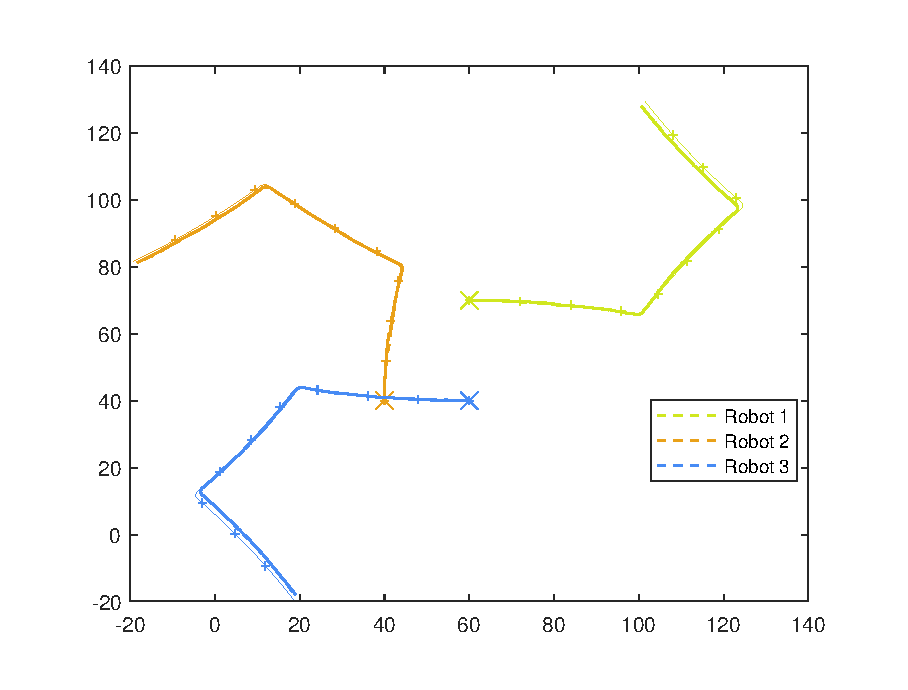
\includegraphics[width=3.7in]{Fig/fig1_traj.eps}
	\caption{Overall trajectory}
	\label{fig::traj}
\end{figure}

Figure \ref{fig::traj} demonstrates their trajectories. The estimated and true lines are overlapping with each other due to small estimation errors.
\begin{figure}
	\centering
	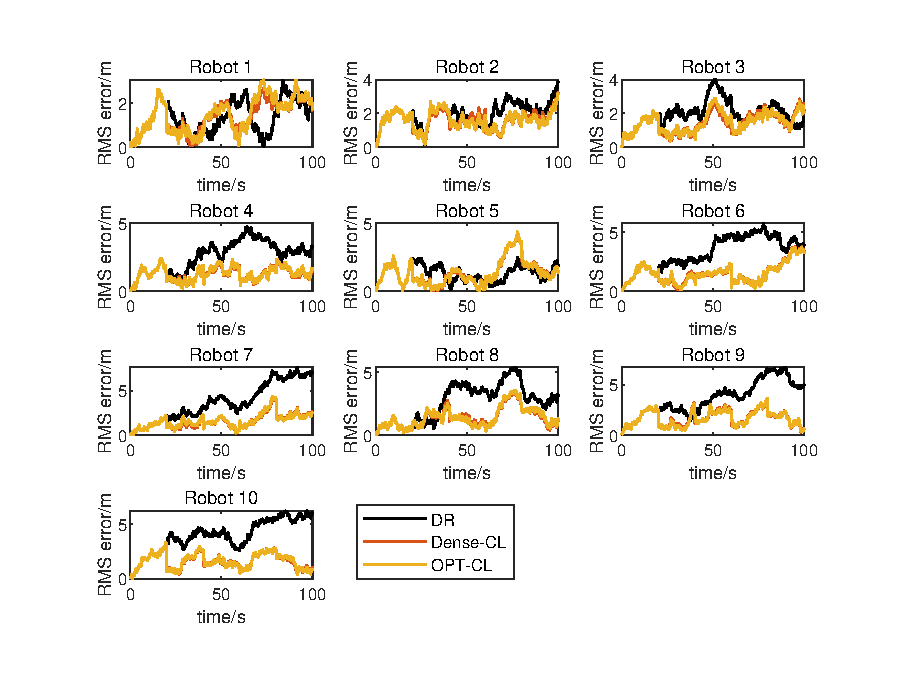
\includegraphics[width=3.7in]{Fig/fig2_rmse.eps}
	\caption{RMS Error}
	\label{fig::rmse}
\end{figure}
Figure \ref{fig::rmse} shows the CEKF, TEKF and SA-TEKF RMS error for all 3 robots, in comparison to dead reckoning (abbreviated as 'DR' in hereafter plot legends).
One can easily see the effectiveness of the CEKF as it dramatically lowers robots' estimation error.
The result of TEKF is also demonstrated, with only small difference compared to that of CEKF.
SA-TEKF has exactly the same position estimation results as TEKF, proving the correctness of our splitting method.
\begin{figure}
	\centering
	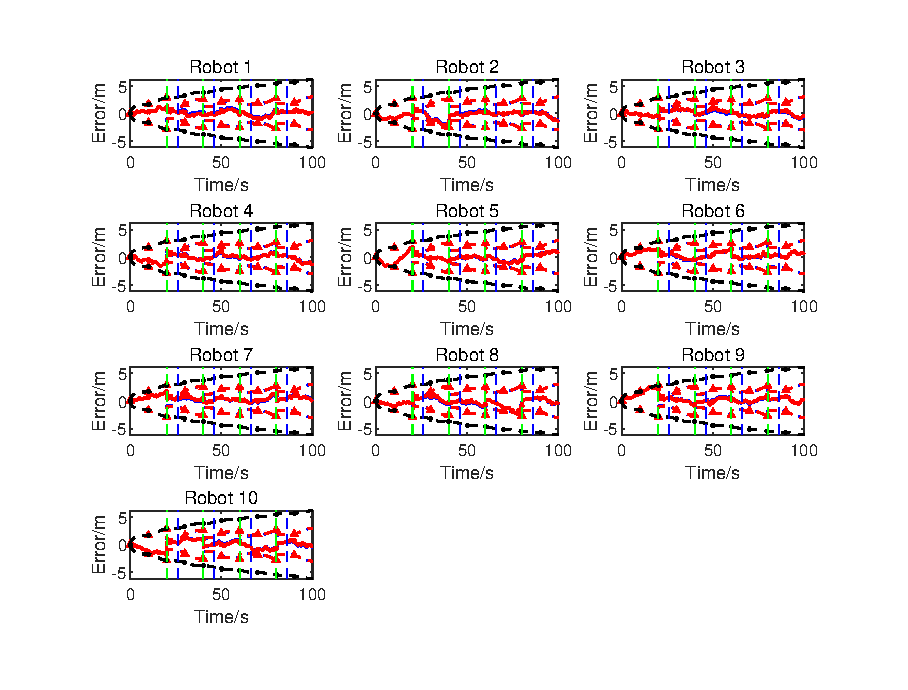
\includegraphics[width=3.7in]{Fig/fig3_3sigma.eps}
	\caption{Three sigma boundaries with estimation errors in X direction}
	\label{fig::3sigma}
\end{figure}

In Figure \ref{fig::3sigma}, three sigma boundaries as well as estimation errors in X direction are displayed.
The black, red, blue and cyan dashed-line are the DR, CEKF, TEKF and SA-TEKF 3-sigma bounds respectively. The red, blue and cyan solid line represents the estimation error of CEKF , TEKF and SA-TEKF, which are all small enough to fit in the 3-sigma bound.
The green and blue dashed-lines stand for the start and end of CL respectively.
As one could see, the covariance of x coordinate estimation is bounded when CL is enabled and it would grow without bound when there is only propagation (DR).
The SA-TEKF has almost the same uncertainty growth as TEKF, with only minor difference when the under-threshold update happens.
\begin{figure}
	\centering
	\subfigure[Trace of covariance (zoomed out)]{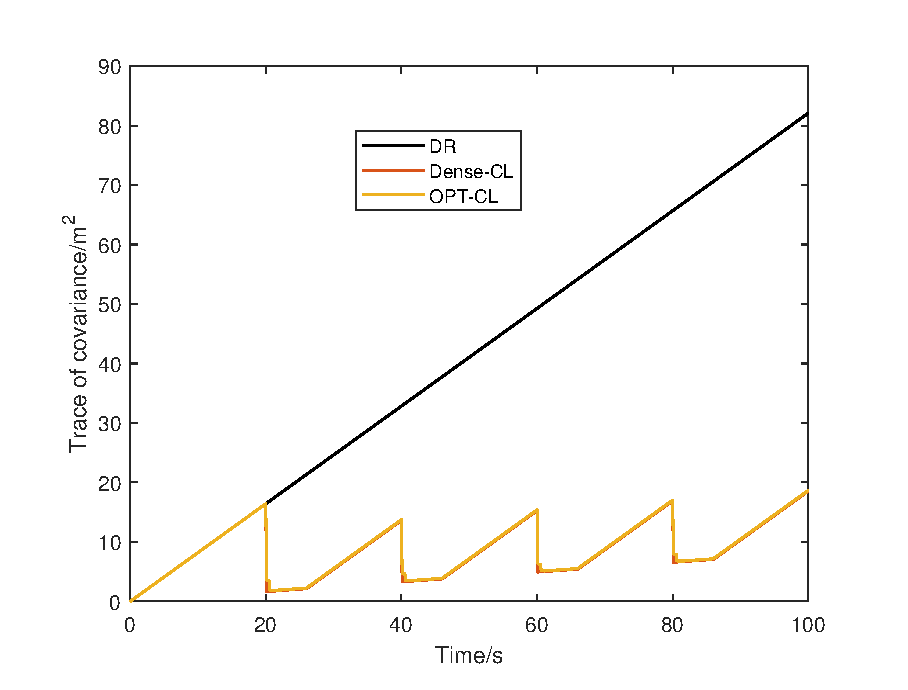
\includegraphics[width=3.7in]{Fig/fig4_trace.eps}}
	\subfigure[Trace of covariance (zoomed in)]{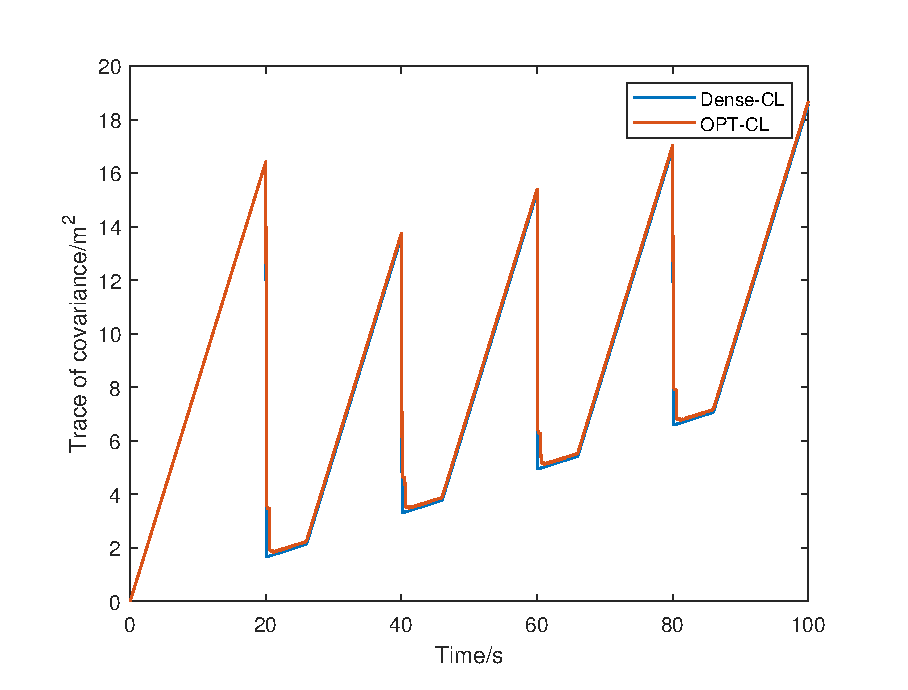
\includegraphics[width=3.7in]{Fig/fig4_trace_zoom_in.eps}}
	\caption{Trace of covariance and its upper bound}
	\label{fig::trace}
\end{figure}

Figure \ref{fig::trace} demonstrates the trace of covariance in multiple methods.
The zoomed out and in figures show that the upper bound given by Eq. \eqref{equ::UB_CEKF} is effective compared with the estimated results by Eq. \eqref{equ::CEKF_main} and by Eq. \eqref{equ::TEKF_update}.
In our simulations, there are 6900 times of communication in CEKF while with $Z = 20I_{2}$, the number for TEKF or SA-TEKF is about 1600, 76.8\% lower.
When the overall system is \emph{observable}, both the CEKF and TEKF/SA-TEKF result in converged estimation uncertainty and its covariance upper bound could be determined. Whenever the CL is turned off and the system becomes \emph{unobservable}, one can clearly observe the unbounded increase of covariance.
The upper bound in blue dashed-line acts as a benchmark for estimation performance comparison as it is the worst-case uncertainty for standard CEKF.
\begin{figure}
	\centering
	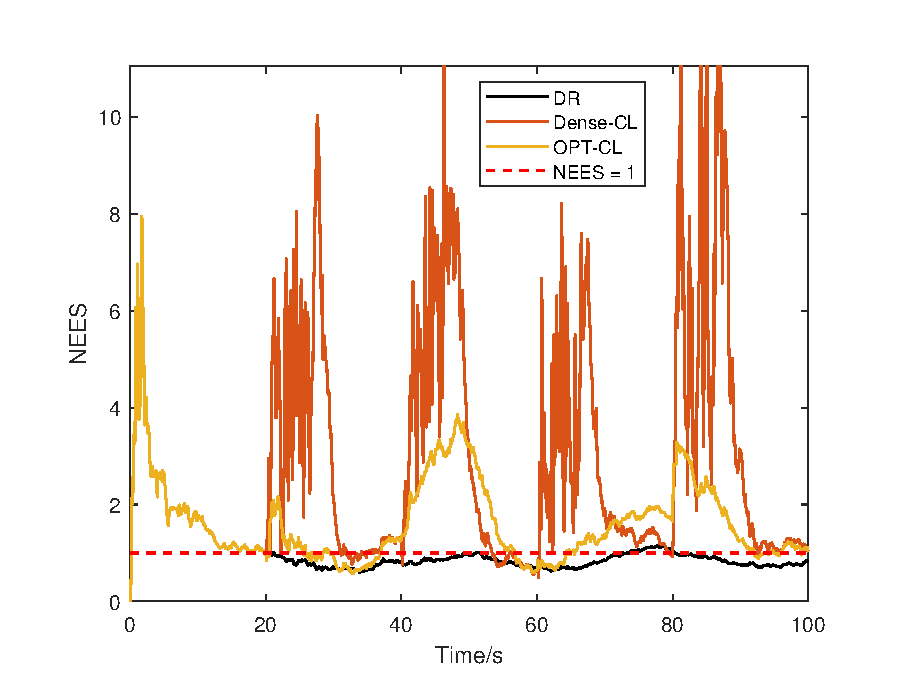
\includegraphics[width=3.7in]{Fig/fig5_nees.eps}
	\caption{NEES comparisons}
	\label{fig::nees}
\end{figure}

Figure \ref{fig::nees} represents the NEES (Normalized Estimation Error Squared) results of different methods. The TEKF or SA-TEKF, with significantly reduced communication costs, yields comparable consistency performance compared to CEKF.

\begin{figure}
	\centering
	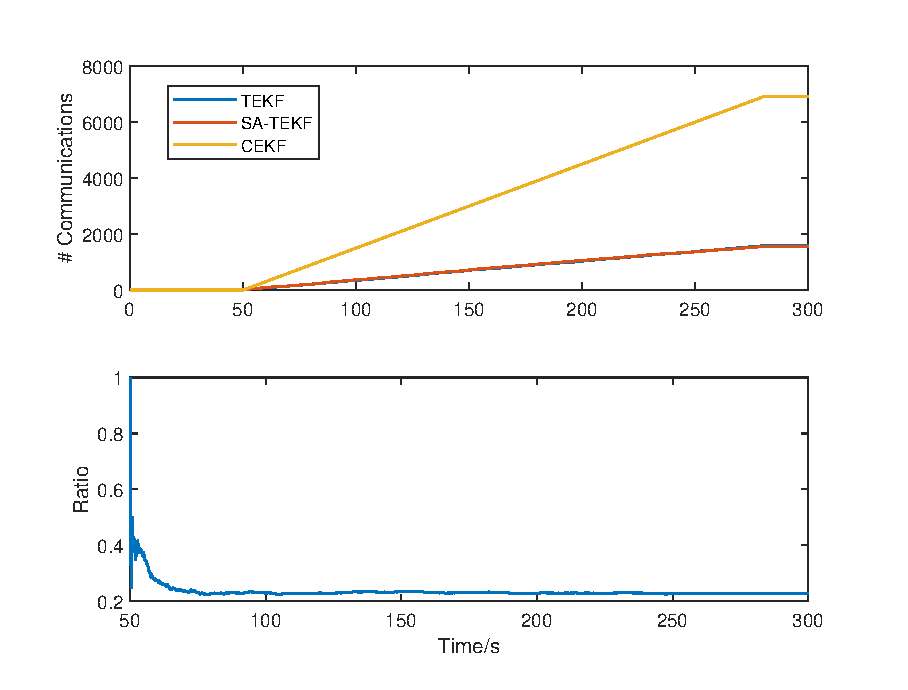
\includegraphics[width=3.7in]{Fig/fig6_com.eps}
	\caption{Communication times comparison}
	\label{fig::com}
\end{figure}
Figure \ref{fig::com} displays the evolution of communication times of SA-TEKF/TEKF and CEKF respectively.
As expected, the SA-TKEF/TEKF has much smaller communication requirements compared to CEKF.

\section{Next to do}
The above results mainly are 1) upper bound derivation and formulation based on discrete-time Riccati recursion equation(DARE), 2) stochastic threshold-based scheduled measurements to reduce server-to-robot communication rate.
I think it might be worthwhile to work on following topics:
\begin{itemize}
	\item Testing the SA-TEKF method on real experimental data in \cite{leung2011utias} (possibly to get a similar result).
	\item Incorporate adjustable observation rate for the optimization problem as in \cite{mourikis2006optimal}.
	One could find the optimal communication rate and observation rate subject to a given total costs dependent on these two rates.
	Actually I haved tried this method in simulation and the result is not very good because the observation rate dominates the overall costs in SA-TEKF method.
	\item Perhaps using another CL fashion other than SA-EKF to make the communication reduction more effectively?
	Since in current method the measurement innovation needs to be calculated at server before deciding transmitting information or not, the \emph{robot-to-server} communication cannot be avoided.
	Only the \emph{robot-to-server} communication could be reduced.
	Multi-centered CL might tackle this problem better?
\end{itemize}

\bibliographystyle{plainnat}
\bibliography{my_ref.bib}
\end{document}


